\section{Experimental API}\label{s:API}

The experimental \ac{API} is designed generically in order to ensure
that it can be used by  applications to maintain dependencies within their
keyspaces irrespective of keyspace schemas or structures of column
families. However, applications using this \ac{API}  have to provide
 the metadata information relevant to the constraints of their keyspace as
 explained in the previous section. 
% Thus,  this \ac{API} is made adaptable to different keyspace schemas  that can
% be deployed in column-oriented key-value \acp{DBMS}.  

This \ac{API} validates the referential integrity based on the metadata provided
for the application and its column families.  It  provides  four solutions
with different approaches to meet different requirements. However, with 
 every one of these solutions,  the referential integrity constraint is
 implemented in Cassandra.

The  class diagram of the \ac{API} is presented seen in
 Figure~\ref{f:classDiagram} alongside with the example classes that belong to 
the University keyspace. The main components are the Entities, Entity Managers,
and Validation handlers, all of which are described in the next sections.  
 Notice that for the sake of clarity and brevity,  the class diagram only
 contains  the relevant  methods of the classes, favoring a simpler
explanation of the functioning of the \ac{API}.

\begin{figure}[h]   
	\centering
	%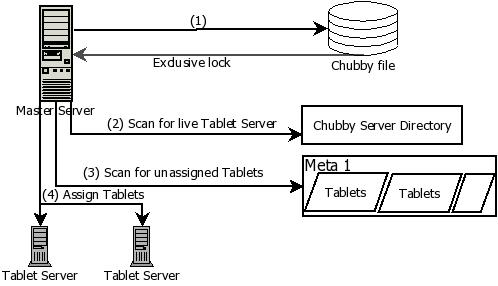
\includegraphics[width=5cm,   height=5cm]{. /figure/random. jpg}
	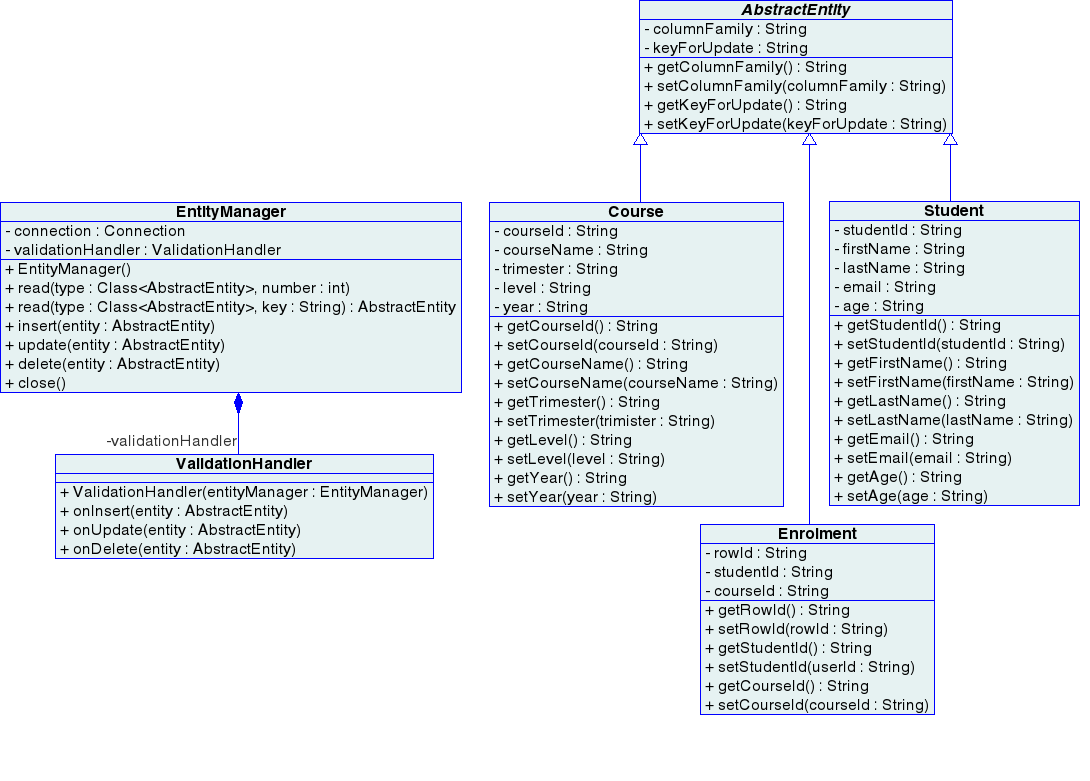
\includegraphics[width=\textwidth]{./figure/Solutions/FinalClassDiagram.png}
	\caption{Class Diagram for the \ac{API}}\label{f:classDiagram}
\end{figure}


	\subsection{Entities} 
	
	An entity class contains attributes (with respective getters and setters) that
	map columns within a specific column family. As such, the contents of a
	column family can be represented by a list of entity objects. All entities in
	the \ac{API} extend from the abstract class \texttt{AbstractEntity} which
	contains attributes (and respective getters and setters) to
	aid the \ac{API} towards their management. Particularly, the attributes
	that \texttt{AbstractEntity} contains  are \texttt{columnFamily} which
	determines the column family to which the entity maps, and 
	\texttt{keyForUpdate} which shall contain the new value in case the primary key
	of the entity is to be updated.
	
	For example,  considering the University keyspace example, \texttt{Enrolment} 
	is an entity class that  maps the \texttt{Enrolment}  column family and
	it contains the attributes \texttt{RowId}, \texttt{CourseId} and
	\texttt{StudentId} which represent the respective columns. As such, an instance
	of \texttt{Enrolment} contains the values of one super column. Likewise,
	\texttt{Student} and \texttt{Course} are entity classes and their instances 
	map to the respective super columns in their column families.
% 	For all the solutions in this \ac{API},  entities of the user applications are
% 	designed to extend the abstract class called \texttt{AbstractEntity},  which has
% 	information about the  methods for accessing and defining  entities.  For
% 	every column family, applications derive a class from the
% 	\texttt{AbstractEntity} containing attributes.
	The \ac{CRUD} operations that can be performed on these entities   are
	handled by the \texttt{EntityManager},  which is described next.
		
	\subsection{EntityManager}

	The  \texttt{EntityManager} class implements  all
	the \ac{CRUD} operations to be performed on the entities. In order to perform
	these operations,  the \texttt{EntityManager} interacts with the respective
	keyspace the entity belongs. Moreover, it ensures to trigger the   referential
	integrity validation process whenever a \ac{CRUD} operation requires it. This
	is performed by creating a  \texttt{ValidationHandler} (explained in the next
	section) and passing the entity to be checked for constraint violations. 
	
	The \texttt{EntityManager}, before performing any operation, requires a
	connection to the keyspace. This connection is established using a third-party
	\ac{API} named Hector (freely available at \todo{www.hector.com}). Hector
	 encapsulates the driver-level interface provided by Cassandra (named Thrift) 
	 and simplifies the interaction with it. Regarding the \ac{CRUD} 
	 operations, Hector provides  a \texttt{Mutator} object which encapsulates the
	 necessary procedures to interact with the Cassandra cluster.    
	 
	 Notice that  the \texttt{EntityManager} is able to generically deal with any
	 entity that derives from \texttt{AbstractEntity}. It does so by using
	 reflection (a Java  feature) to detect the attributes of an object and
	 generically invoking the getters and setters of the entities. Thus, the
	 \texttt{EntityManager} is able to perform all \ac{CRUD} operations on
	 any entity. These operations are explained in detail next.  
	 
	 
	
% 	Hector is a high
% 	 level client that wraps the driver-level interface of Cassandra called Thrift.
% 	 Hector  provides some features that  Thrift does not, for example, 
% 	 fail-over mechanisms and connection pooling (\todo{cite book}).  
	 % 	 While there
% 	 are other wrappers for Thrift, Hector was  chosen as  it is one of the
% 	 earliest wrappers and  encapsulates the interaction with the Thrift \ac{API}
% 	 and makes it simpler to access a Cassandra cluster.	
	
	
	
	
		\subsubsection{Create}
		 The \texttt{create} (or \texttt{insert}) operation stores entities in the
		 respective column families. The \texttt{EntityManager} inserts these entities
		into the column families represented by the entity class.  
		For example,  all the student entities are inserted into the column family
		\texttt{Student} through the \texttt{EntityManager}. 
		
		The \texttt{EntityManager} passes the entity details which include entity key
		and column family information as parameters to the \texttt{addInsertion}
		method of the \texttt{Mutator}.  The \texttt{insert} operation triggers a
		 referential integrity validation whenever a child entity is  inserted in
		 order to ensure that its parent entities exist. The validation is performed
		 by the \texttt{onInsert} method of \texttt{ValidationHandler}, which is
		explained in Section~\ref{ss:VH}.
	
		\subsubsection{Read}
		The  \texttt{read} operation retrieves  entities from a keyspace given the
		entity class. This operation does not prompt any referential integrity validation since
 		entities are only read and their state is not changed, unlike in the other
		operations.
		
% 		\todo{talk about mutator CONSISTENCY}
		
		This \ac{API} provides two methods for retrieving entities. One retrieves a
		single entity given its class and the value of the respective primary key. The
		other retrieves a list of entities representing the contents of
		the column family.

		
		
		\subsubsection{Update}\label{ss:update}
		In an \texttt{update} operation the existing contents of an entity are merged
		with new contents.  In other words, the  values of their columns they
		represent are updated to new values and committed into the column families.  
		 The \texttt{EntityManager} provides two types of updates, one in which it
		 uses the primary key of the entity to update it, and the other one in
		 which uses the especial field \texttt{keyForUpdate} to update the primary as
		 well as the rest of the fields. 
		 
		 If the entity to be updated does not contain a change in its primary key, a
		 normal update takes place. Otherwise, referential integrity needs to be
		 ensured. In order to do so, the following steps are performed:
% 		 In order to do so, the \texttt{EntityManager} passes the entity
% 		 to the \texttt{ValidationHandler}  to check for referential integrity, 
% 		 retrieves the list of child entities that depend on its primary key, deletes
% 		 dependencies and the entity,  and update the dependencies Following this, the
% 		 steps that are performed are :
		\begin{enumerate}
		  \item Check with the \texttt{ValidationHandler} if the entity can be
		  updated.
		  \item Retrieve the list of child entities that depend on the previous
		  primary key of the entity to be updated.
		  \item Perform \texttt{delete} on the child entities from their column family
		  in Cassandra.
		  \item Perform a \texttt{delete} on the entity with the primary key from the
		  column family.
		  \item Perform an \texttt{insert} with the entity and its new primary key.
		  \item Update the foreign keys in the child dependencies to
		  the new value.
		  \item Perform an \texttt{insert} operation to reinsert the child entities
		  into their respective column families.
		\end{enumerate}
		
% 		In all the solutions,  an \texttt{Update} operation triggers a referential
% 		 integrity validation whenever any primary or foreign keys of any entities are
% 		updated.
% 		The validations are performed by the \texttt{onUpdate} method of the
% 		\texttt{ValidationHandler}.
		
		Notice that such procedure is used as a workaround of the restriction of
		Cassandra to change a primary key. Once a record has been
		inserted into the column family, the primary key cannot  be changed. This is
		known as a tombstone delete, which prevents aside from changing a primary
		key, deleting a primary key.
		
		\subsubsection{Delete}\label{ss:delete}
		In a  \texttt{Delete} operation, entities are removed from a column
		family. As mentioned before, due to the tombstone delete, the primary key
		will never cease to exist, but the values of the columns are emptied. 
		
		In all the solutions,  a \texttt{Delete} operation triggers a referential
		integrity validation every time a parent entity is deleted.  This validation
		is performed by the \texttt{onDelete} method of the
		\texttt{ValidationHandler}, which is explained in next section. 
		 
		 The 	\texttt{EntityManager} passes the entity information to the
		\texttt{delete} method of the \texttt{Mutator} object.
 		
%  		Before a parent entity is deleted, the \texttt{EntityManager} retrieves the
%  		child entities it depends upon  from he \texttt{ValidationHandler} if the
%  		 referential intergity is not violated. The \texttt{EntityManager} deletes
%  		the child entities prior to deleting the parent entity.
		
		\subsection{ValidationHandler}\label{ss:VH}
		The \texttt{ValidationHandler} is invoked by the \texttt{EntityManager} every time
		an operation triggers a
		referential integrity validation on any entity. 
		The \texttt{EntityManager} passes the entity and the connection details  to
		the \texttt{ValidationHandler} to perform the validation.
		
		The \texttt{ValidationHandler} contains the  logic for checking whether an
		 entity has any dependencies and verifies whether an \texttt{insert},
		 \texttt{update} or \texttt{delete} operation  violates the referential
		integrity or not.  To ensure that these operations maintain referential
		 integrity between entities, it applies the appropriate referential integrity
		 rules, as explained in Section~\ref{s:referential-integrity}. Thus, for an
		 \texttt{insert} operation the insert rule of referential integrity is
		 followed and similarly for \texttt{update} and \texttt{delete} operations
		 their respective rules are applied. As previously mentioned, a \texttt{read}
		 operation does not invoke any referential integrity validation in this
		 \ac{API}. The referential integrity validation performed by
		 \texttt{ValidationHandler} for each of these operations is discussed next
		with pseudocodes.
		
		\begin{description}
		\item[onInsert]: 
		In an \texttt{insert} operation a referential
		integrity validation is triggered whenever a child entity is  inserted. 
		The \texttt{ValidationHandler} applies the referential integrity insert
		rule which checks whether  valid parent entities with
		primary keys matching the foreign keys of the child entities exist, else an
		exception is raised stating that the referential integrity has been violated.
		Thus, the following checks are performed by the \texttt{ValidationHandler}.
		\renewcommand{\labelenumii}{\arabic{enumi}.\arabic{enumii}}
		\renewcommand{\labelenumiii}{\arabic{enumi}.\arabic{enumii}.\arabic{enumiii}}
		
		\begin{enumerate}
		\item if entity has \ac{FK} constraints
				\begin{enumerate}
				\item Identify parent entity class from the \ac{FK} constraint.
				\item if foreign keys exist as  primary key in  parent entity class
				  		\begin{enumerate}
				  		\item \texttt{EntityManager} inserts the entity.
				  		\end{enumerate}
				\item else
				   		\begin{enumerate}
				   		  \item Raise exception and cancel \texttt{insert}.
				   		\end{enumerate}
				\end{enumerate}   	
		\item else if no \ac{FK} constraints exist
		  		\begin{enumerate}
		  		\item \texttt{EnityManager} inserts entity.
		  		\end{enumerate}
		\end{enumerate}
		The implementation of the \texttt{insert} operation is consistent across all the
		solutions. 
		\item[onUpdate:] The validation for an \texttt{update} operation is different
		when primary keys and foreign keys are updated. 
		\begin{description}
		\item[Case A: Update Primary Key] When a  primary key of a
		parent entity is updated, the \texttt{ValidationHandler} performs the
		following checks.
		\renewcommand{\labelenumii}{\arabic{enumi}.\arabic{enumii}}
		\renewcommand{\labelenumiii}{\arabic{enumi}.\arabic{enumii}.\arabic{enumiii}}
		%\renewcommand{\labelenumiiii}{\arabic{enumi}.\arabic{enumii}.\arabic{enumiii}.\arabic{enumiiii}}
		\begin{enumerate}
		  \item if \ac{FK} constraints on primary key exist
		  	\begin{enumerate}		  	
		    \item if \texttt{DeleteRule} for the \ac{FK} constraint is
		    \texttt{Cascade}
		    	\begin{enumerate}
		    	  \item Pass any existing child entities to the \texttt{EntityManager} to
		    	  allow update of both primary and foreign keys.
				\end{enumerate}
			\item else if \texttt{DeleteRule}  is \texttt{NoDelete}
				\begin{enumerate}
				  \item if no child entities exist
				  		\begin{enumerate}
				  		  \item \texttt{EntityManager} performs update on  the primary key.
				  		\end{enumerate}
				  \item else if child entities exist
				   		\begin{enumerate}
				    	\item Raise exception and rollback \texttt{update}. 
				    	\end{enumerate}
				\end{enumerate}
			\end{enumerate}
		  \item else if no \ac{FK} constraints are found 
		  		\begin{enumerate}
		  		  \item \texttt{EntityManager} performs update on the primary key.
				\end{enumerate}
		 \end{enumerate}
		 
		For example,  in the University keyspace,  when a
		new \texttt{StudentId} is provided for an existing  \texttt{Student}
		entity,  then \texttt{ValidationHandler}
		checks metadata and locates the \ac{FK} constraint \texttt{CONST400} as seen in
		Figure~\ref{f:metadataInSolutions}. Since the \texttt{DeleteRule} is
		\texttt{Cascade}, the \texttt{EntityManager} allows the \texttt{update}
		operation to take place as explained in the EntityManager section.
			
% 			For example, when the foreign key \texttt{StudentId} for one of the entities
% 		in \texttt{Enrolment} is given a new value,  then the \texttt{ValidationHandler} 
% 		identifies the parent entity class for its \ac{FK} constraint
% 		\texttt{CONST400} as \texttt{Student}.  If the new \texttt{StudentId} 
% 		exists as a primary key for any
% 		 of the  entities in \texttt{Student} entity class,  the \texttt{update} is
% 		 performed.
		 
		\item[Case B: Update Foreign Key] When a foreign key of a child entity is
		updated, the  \texttt{EntityManager} performs the same check on the
		metadata and locates its \ac{FK} constraints. It then follows these steps:
		\begin{enumerate}
		  \item Identify parent entity class from the \ac{FK} constraint.
		  \item if new foreign keys exist as primary key in parent entity class
			\begin{enumerate}
				\item \texttt{EntityManager} updates  the foreign key.
			\end{enumerate}
		  \item else 
			\begin{enumerate}
				\item Raise exception.
			\end{enumerate}
		\end{enumerate}

	
		
		\end{description}
		The implementation of the \texttt{update} operation for both the cases is
		consistent for all solutions.
		
		\item[onDelete:] In a \texttt{delete} operation a referential
		integrity validation is triggered whenever an entity is deleted. The
		\texttt{ValidationHandler} applies the referential integrity delete rule
		and performs the following checks:
		\renewcommand{\labelenumii}{\arabic{enumi}.\arabic{enumii}}
		\renewcommand{\labelenumiii}{\arabic{enumi}.\arabic{enumii}.\arabic{enumiii}}
		
		\begin{enumerate}
		  \item Identify existing \ac{FK} constraints on the entity.
		  \item if \ac{FK} constraints exist,
		  		\begin{enumerate}
		  		  \item if \texttt{DeleteRule} is \texttt{Cascade}
		  		 		\begin{enumerate}
		  		 		   \item Pass any existing child entities to the \texttt{EntityManager}
		  		 		   to allow delete of child  and parent entities.
		  		 		\end{enumerate}
		  		  \item else if \texttt{DeleteRule}  is \texttt{NoDelete}
						\begin{enumerate}
						  \item if no child entities exist
						  		\begin{enumerate}
						  		  \item \texttt{EntityManager} deletes the entity.
						  		\end{enumerate}
						  \item else if child entities exist
						   		\begin{enumerate}
						    		\item Raise exception. 
						    	\end{enumerate}
						\end{enumerate}
						
				  \item else if no \ac{FK} constraints are found 
				  		\begin{enumerate}
				  		  \item \texttt{EntityManager} deletes the entity.
						\end{enumerate}
		  		\end{enumerate}
		\end{enumerate}	
		For example,  in the University keyspace,  if a 
		\texttt{Student} entity in \texttt{Student} column family is marked for
		deletion, the \texttt{EntityManager} locates the \ac{FK} constraint 
		\texttt{CONST400} referencing \texttt{Student}.
		Since the \texttt{DeleteRule} is \texttt{Cascade}, 
		the child entities are deleted from \texttt{Enrolment} prior to deleting the
		entity from its \texttt{Student} column family. 
		\end{description}
		
% 		
% 		Since metadata is stored differently in the solutions, the operation for
% 		retrieving the metadata in the  \texttt{ValidationHandler} is different for
% 		each solution in the \ac{API}. 
% 		 For example,  the \texttt{ValidationHandler}
% 		for Solution 1 and 2 involves parsing the metadata  since it is stored as a
% 		 \texttt{String} along with the actual data while in Solution 3 and 4 it is
% 		 saved as an entity class.
% 		
		The referential integrity validation logic, implementation of the \ac{CRUD}
		operations and Cassandra connection settings are common for all the solutions
		in the \ac{API}.
		
		The following sections describe each of the four solutions in terms of how
		these store ,decipher, access and retrieve the metadata. The motivation for
		each of the solution is also discussed. 
% 		how metadata is accessed and retrieved
% 		and the motivation for the solution's design.

